\documentclass[a4paper]{article}
%\VignetteIndexEntry{UP - unequal probability sampling designs}
%\VignettePackage{sampling}
\newcommand{\sampling}{{\tt sampling}}
\newcommand{\R}{{\tt R}}
\setlength{\parindent}{0in}
\setlength{\parskip}{.1in}
\setlength{\textwidth}{140mm}
\setlength{\oddsidemargin}{10mm}
\title{Unequal probability sampling designs}
\author{}
\usepackage{Sweave} 
\usepackage[latin1]{inputenc}
\usepackage{amsmath}



\begin{document}
\maketitle

1) Some examples of using maximum entropy sampling design and related functions:

a) First example

Sample of Belgian municipalities, sample size 50

\begin{Schunk}
\begin{Sinput}
> data(belgianmunicipalities)
> attach(belgianmunicipalities)
> n=50
\end{Sinput}
\end{Schunk}
Inclusion probabilties proportional to the 'averageincome' variable

\begin{Schunk}
\begin{Sinput}
> pik=inclusionprobabilities(averageincome,n)
\end{Sinput}
\end{Schunk}
Draw a sample

\begin{Schunk}
\begin{Sinput}
> s=UPmaxentropy(pik)
\end{Sinput}
\end{Schunk}
The sample is

\begin{Schunk}
\begin{Sinput}
> as.character(Commune[s==1])
\end{Sinput}
\end{Schunk}
Joint inclusion probabilities

\begin{Schunk}
\begin{Sinput}
> pi2=UPmaxentropypi2(pik)
\end{Sinput}
\end{Schunk}
Check the result

\begin{Schunk}
\begin{Sinput}
> rowSums(pi2)/pik/n
\end{Sinput}
\end{Schunk}
b) Second example

Selection of samples from Belgian municipalities data, sample size 50.
Once matrix q is computed, a sample is quickly selected.
Simulations can be run to compare the results.
 
\begin{Schunk}
\begin{Sinput}
> data(belgianmunicipalities)
> attach(belgianmunicipalities)
> pik=inclusionprobabilities(averageincome,50)
> pik=pik[pik!=1]
> n=sum(pik)
> pikt=UPMEpiktildefrompik(pik)
> w=pikt/(1-pikt)
> q=UPMEqfromw(w,n)
\end{Sinput}
\end{Schunk}
Draw a sample using the q matrix

\begin{Schunk}
\begin{Sinput}
> UPMEsfromq(q)
> 
\end{Sinput}
\end{Schunk}
Simulations to check the sample selection; the difference between pik and the computed inclusion prob. tt is almost 0.

\begin{Schunk}
\begin{Sinput}
> sim=10000
> N=length(pik)
> tt=rep(0,N)
> for(i in 1:sim) tt = tt+UPMEsfromq(q)
> tt=tt/sim
> max(abs(tt-pik))
\end{Sinput}
\end{Schunk}
2) This is an example of unequal probability (UP) sampling functions: selection of samples using the Belgian municipalities data set,
with equal or unequal probabilities, and study of the Horvitz-Thompson estimator accuracy using boxplots. The following
sampling schemes are used: Poisson, random systematic, random
pivotal, Till\'e, Midzuno, systematic, pivotal, and simple random
sampling without replacement. Monte Carlo simulations are used to study the accuracy of the
Horvitz-Thompson estimator of a population total. The aim of this
example is to demonstrate the effect of the auxiliary information incorporation in the sampling design. We use:
\begin{itemize}
\item some $\pi$ ps sampling designs with Horvitz-Thompson estimation,
using in the sampling design the information on size measures of
population units;
\item simple random sampling without replacement with Horvitz-Thompson
estimation, where no auxiliary information is used.
\end{itemize}

\begin{Schunk}
\begin{Sinput}
> b=data(belgianmunicipalities)
> pik=inclusionprobabilities(belgianmunicipalities$Tot04,200)
> N=length(pik)
> n=sum(pik)
\end{Sinput}
\end{Schunk}
Number of simulations (for an accurate result, increase this value to 10000):

\begin{Schunk}
\begin{Sinput}
> sim=10
> ss=array(0,c(sim,8))
\end{Sinput}
\end{Schunk}
Defines the variable of interest:

\begin{Schunk}
\begin{Sinput}
> y=belgianmunicipalities$TaxableIncome
\end{Sinput}
\end{Schunk}
Simulation and computation of the Horvitz-Thompson estimator:

\begin{Schunk}
\begin{Sinput}
> ht=numeric(8)
> for(i in 1:sim)
+ {
+ cat("Step ",i,"\n")
+ s=UPpoisson(pik)
+ ht[1]=HTestimator(y[s==1],pik[s==1])
+ s=UPrandomsystematic(pik)
+ ht[2]=HTestimator(y[s==1],pik[s==1])
+ s=UPrandompivotal(pik)
+ ht[3]=HTestimator(y[s==1],pik[s==1])
+ s=UPtille(pik)
+ ht[4]=HTestimator(y[s==1],pik[s==1])
+ s=UPmidzuno(pik)
+ ht[5]=HTestimator(y[s==1],pik[s==1])
+ s=UPsystematic(pik)
+ ht[6]=HTestimator(y[s==1],pik[s==1])
+ s=UPpivotal(pik)
+ ht[7]=HTestimator(y[s==1],pik[s==1])
+ s=srswor(n,N)
+ ht[8]=HTestimator(y[s==1],rep(n/N,n))
+ ss[i,]=ht
+ }
\end{Sinput}
\end{Schunk}
Boxplots of the estimators:

\begin{Schunk}
\begin{Sinput}
> colnames(ss) <- 
+ c("poisson","rsyst","rpivotal","tille","midzuno","syst","pivotal","srswor")
> boxplot(data.frame(ss), las=3)
> 
\end{Sinput}
\end{Schunk}
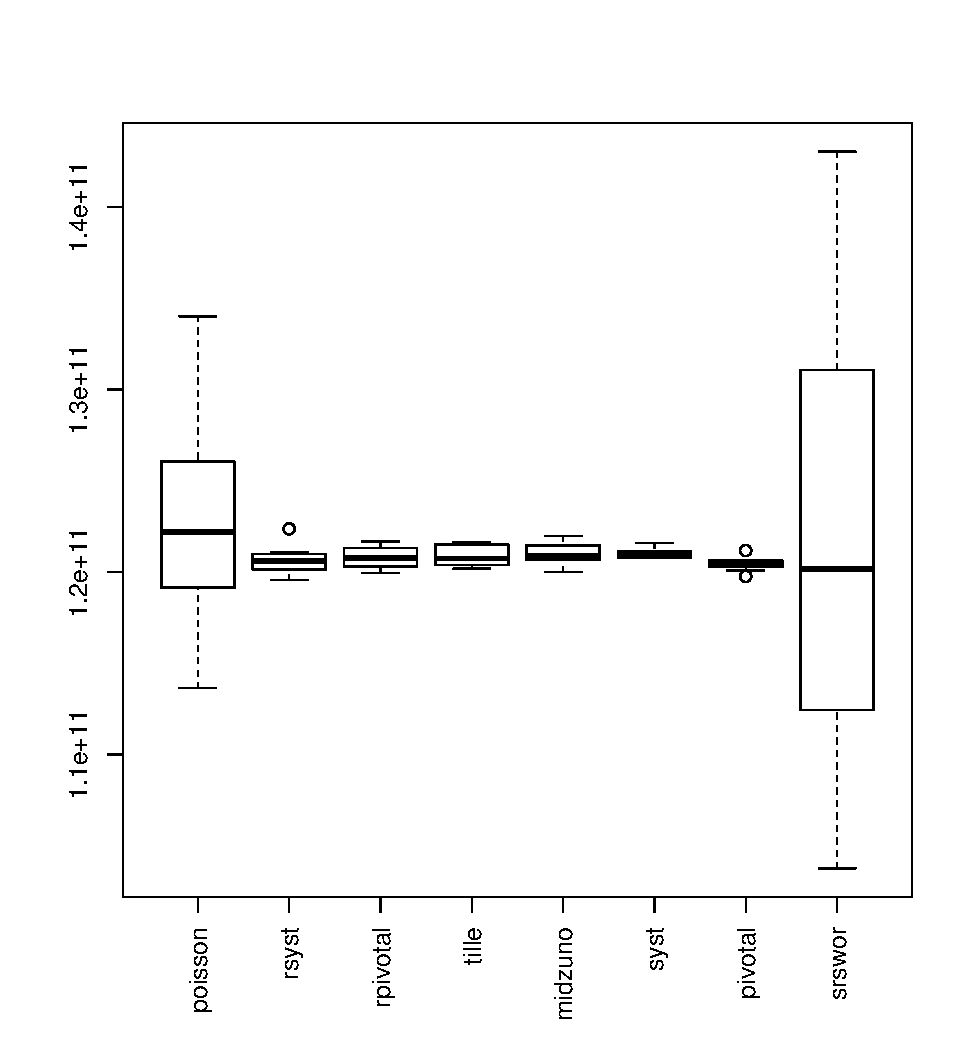
\includegraphics{UPexamples-up5}
\end{document}
